\part{Ejercicio 3}
\section{Enunciado}
Un radix tree o PATRICIA es un trie en el cual las cadenas de nodos con un solo hijo
son compactadas y transformadas en un solo nodo. Esto permite mejorar el consumo de
memoria de la estructura en el caso en que hay pocas cadenas definidas o que muchas
cadenas tengan prefijos largos en com'un.
Esta compactaci'on genera entonces las diferencias b'asicas entre los radix trees y los tries:
a) Todos los nodos internos de un radix tree tienen como m'inimo dos hijos (excepto
posiblemente la raiz).
b) Las ramas de un radix tree pueden estar etiquetadas con m'as de un caracter.
Si adem'as el conjunto (o del conjunto de claves del diccionario) es un conjunto libre
de prefijos, sucede que las cadenas (o los valores asociados a las claves) se encuentran
solamente en las hojas. Un conjunto libre de prefijos es aquel en el cual ningun elemento
es prefijo de otro.
Implementar un conjunto de cadenas basado en estas ideas que soporte las siguientes
operaciones:
a) Agregar una cadena al conjunto.
b) Consultar si una cadena pertenece al conjunto.
c) Sacar una cadena del conjunto.
d) Consultar la cantidad de cadenas del conjunto.
Donde las cadenas forman un conjunto libre de prefijos. Las tres primeras operaciones
deben tener complejidad O(ksk) donde s es la clave m'as larga ya definida y ksk indica la
longitud de s. La 'ultima operaci'on debe tener complejidad de orden constante.
El conjunto de caracteres sobre el que se van a definir las cadenas son las 26 letras min'uscu-
las del ingl'es.

\section{Desarrollo}
\subsection{PATRICIA}
Un Radix Tree o PATRICIA (Practical Algorithm To Retrieve Information Coded In Alphanumeric) es una estructura de datos basada en los Tries que cumple el rol de diccionario. Sus claves son cadenas, y su significado es de tipo variado, d'andole uso para diferentes prop'ositos. La diferencia entre un PATRICIA y un Trie ya fue mencionada en el enunciado: un trie tiene un nodo por cada caracter de ua cadena, en cambio las ramas de un radix tree pueden estar etiquetadas con m'as de un caracter, y si adem'as el conjunto de claves es libre de prefijos, cada nodo del radix tendr'a almenos dos hijos.

\subsection{Sobre el dise\~{n}o de la estructura}
Por sus caracter'isticas, el PATRICIA presenta un amplio abanico de posibles implementaciones. Nosotros basicamente pensamos en tres formas:
\begin{itemize}
\item Con nodos formados por un arreglo (en este caso de 26 posiciones) que tiene ejes por elementos
\item con nodos formados por una lista de ejes 
\item con nodos que contienen una tabla de hash
\end{itemize}
Un eje es una tupla de puntero a un nodo hijo y una cadena adjunta. Los nodos pueden tener un bit que indica la validez o invalidez del mismo y/o el dato (significado) a guardar. En el caso de este TP, no se piden datos a guardar, por lo tanto optamos por implementar los nodos con dos variantes de las ya nombradas: nodos formados por un arreglo de 26 posiciones con un bit de existencia y nodos formados por una lista con un bit de existencia. Como luego veremos, ambos dise\~{n}os de estructura cumplir'an las complejidades pedidas. El bit de existencia permite que podamos usar el patricia aun en casos donde el conjunto de entrada no este libre de prefijos, por ejemplo consideremos la figura \ref{fig:bitExistencia} en este caso si bien la forma del PATRICIA es la misma, mediante el bit de existencia podemos diferenciar si la palabra `emi' esta o no definida.
\begin{figure}[H]
\centering
\subfigure[La palabra emi no esta definida]{
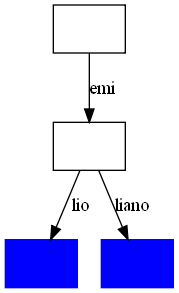
\includegraphics[scale=0.5]{./figuras/ej3/bitDeExistencia.png} }\hspace{1in} 
\centering
\subfigure[La palabra emi si esta definida]{
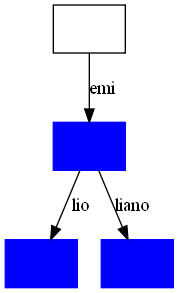
\includegraphics[scale=0.5]{./figuras/ej3/bitDeExistencia1.png} }
\setcounter{subfigure}{0}
\caption{Utilizaci�n del bit de existencia}
\label{fig:bitExistencia}
\end{figure}

En cuanto al PATRICIA, se decidi'o que el mismo contendr'a nodos y no los definir'a dentro. O sea, separamos el objeto 'arbol PATRICIA del objeto nodo. Esto es as'i pues de este modo se implementa la modularidad que resulta de gran utilidad para implementar el PATRICIA para los diferentes tipos de nodo.

\subsection{Sobre el PATRICIA como 'arbol}
El enunciado presenta un invariante para el PATRICIA: 
\begin{itemize}
\item Todos los nodos internos de un radix tree tienen como m'inimo dos hijos (excepto
posiblemente la raiz).
\item Si adem'as el conjunto (o del conjunto de claves del diccionario) es un conjunto libre
de prefijos, sucede que las cadenas (o los valores asociados a las claves) se encuentran
solamente en las hojas. Un conjunto libre de prefijos es aquel en el cual ningun elemento
es prefijo de otro.
\end{itemize}
Este invariante deber'a conservarse durante todas las funciones.
El diccionario PATRICIA nos sugiere un 'arbol formado de un conjunto de palabras dispersas en su estructura, como muestra el siguiente gr'afico.

\begin{figure}[H]
\centering
\includegraphics[scale=0.5]{./figuras/e3/patricia.png}
\caption{Ejemplo de �rbol patricia}
\end{figure}

Los nodos azules representan a las claves definidas. Este 'arbol se va formando a medida que agregamos y sacamos palabras del conjunto de claves. A continuaci'on describiremos cuales fueron las pautas a seguir para armar dichas funciones.

\subsection{Agregando un elemento}
Cuando agregamos un elemento nos enfrentamos ante los siguientes casos:
\begin{itemize}
\item Se puede agregar el elemento sin tener que partir un eje

\begin{figure}[H]
\centering
\subfigure[PATRICIA original]{
\includegraphics[scale=0.4]{./figuras/ej3/patricia.png} }
\centering
\subfigure[ ]{
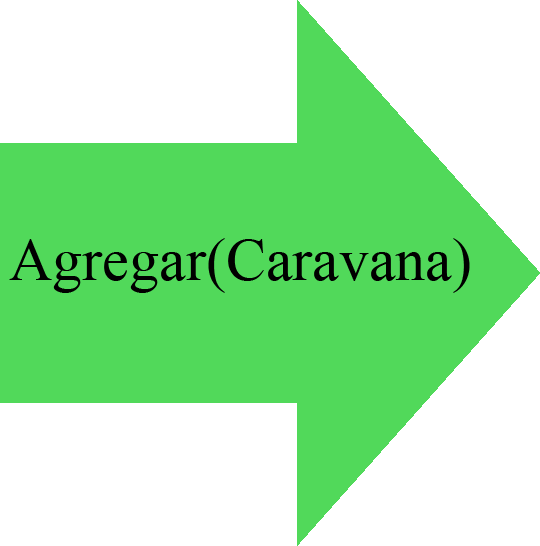
\includegraphics[scale=0.2]{./figuras/ej3/arrow.png} }
\centering
\subfigure[Bajamos lo m'aximo posible]{
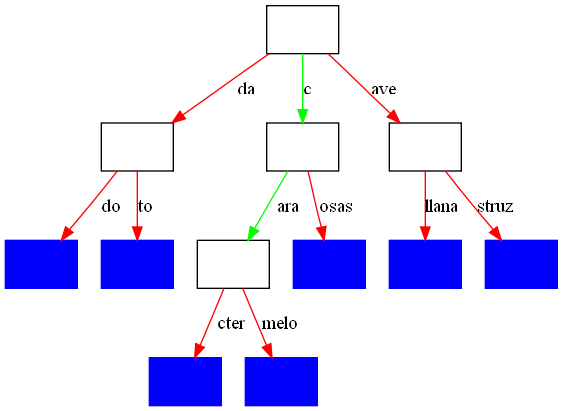
\includegraphics[scale=0.4]{./figuras/ej3/patriciaCaravanaBajando.png} }
\centering
\subfigure[Patricia luego de agregar caravana]{
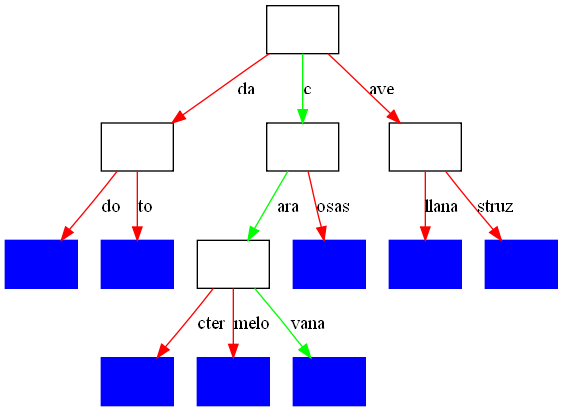
\includegraphics[scale=0.4]{./figuras/ej3/patriciaCaravana.png} }
\setcounter{subfigure}{0}
\caption{}
\label{fig:noPartirNodo}
\end{figure}

\item Para agregar un elemento, hay que partir un eje y agregar un nodo

\begin{figure}[H]
\centering
\subfigure[PATRICIA original]{
\includegraphics[scale=0.4]{./figuras/ej3/patricia.png} }
\centering
\subfigure[ ]{
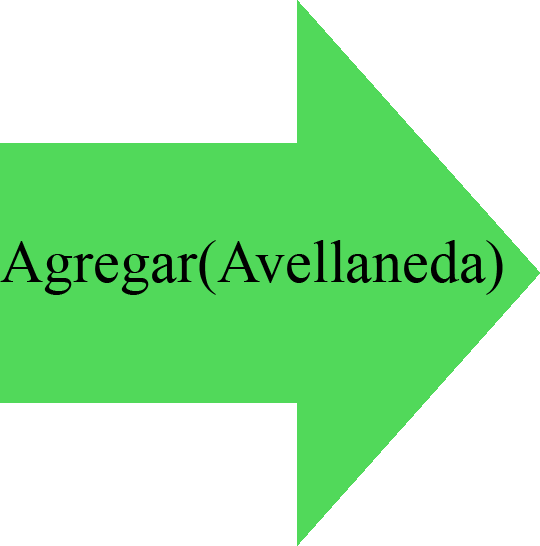
\includegraphics[scale=0.2]{./figuras/ej3/arrow2.png} }
\centering
\subfigure[Tenemos que partir el nodo de llana]{
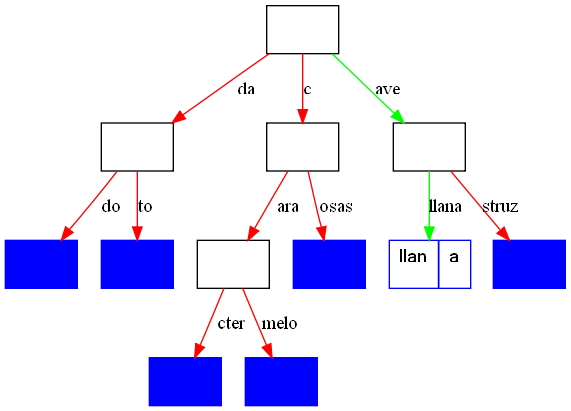
\includegraphics[scale=0.4]{./figuras/ej3/partiendoNodo.png} }
\subfigure[Ahora que lo partimos podemos agregar la palabra como en el caso anterior]{
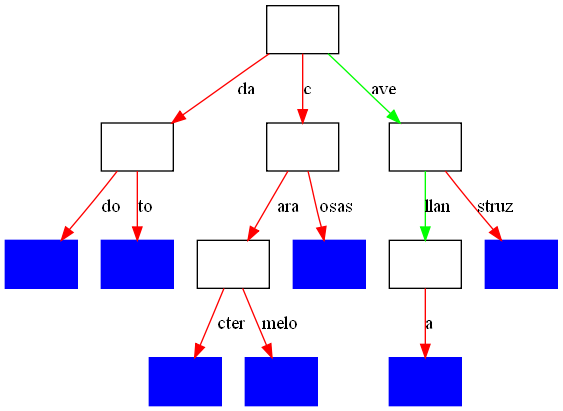
\includegraphics[scale=0.4]{./figuras/ej3/NodoPartido.png} }
\subfigure[Patricia luego de agregar avellaneda]{
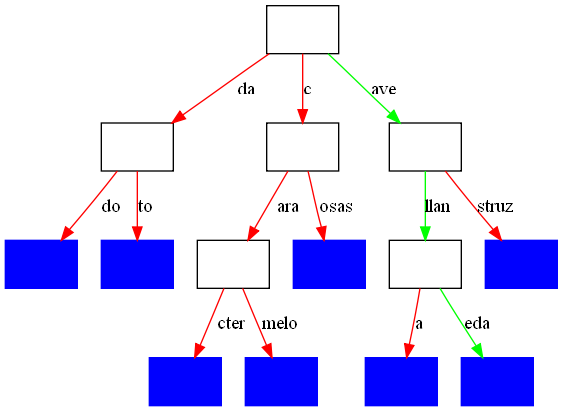
\includegraphics[scale=0.4]{./figuras/ej3/patriciaAvellaneda.png} }
\setcounter{subfigure}{0}
\caption{}
\label{fig:partirNodo}
\end{figure}

\end{itemize}

Para solucionar estos casos comenzaremos situ'andonos sobre la ra'iz. Luego bajamos por las ramas de la siguiente manera: en cada paso mantenemos guardada la palabra formada a partir de la concatenacion de las cadenas adjuntas de los ejes por los cuales baj'e, y la cadena recortada que resulta de quitarle a la clave el prefijo en com'un que tiene con cada eje por el cual baj'e. De esta forma en cada paso buscamos el eje tal que la primer letra de su cadena adjunta coincida con la primer letra de palabra recortada. As'i bajaremos por los ejes hasta que encontremos un eje que no sea prefijo, en su totalidad, de la cadena recortada, como se muestran los dos casos en las figuras \ref{fig:noPartirNodo}c y \ref{fig:partirNodo}c. Este algoritmo no presenta ambiguedades a la hora de buscar el eje por el cual bajar, pues cada nodo tiene un m'aximo de 26 hijos, correspondientes a las 26 letras del abecedario ingl'es, y no puede tener mas de un eje que su cadena adjunta comience con la misma letra. O sea, no puede haber nodos con, por ejemplo, ejes con cadenas casa y cosa.
Una vez que bajamos por las ramas lo m'aximo posible, si la palabra formada es prefijo de la clave a definir, quiere decir que caimos en el primer caso. Este caso es simple y solo resta agregar el nodo y el eje correspondiente, con la clave sin prefijo, como se muestra en la figura \ref{fig:noPartirNodo}, gr'afico d.
Supongamos ahora que se desea agregar \"avellaneda\". Bajamos por las ramas. Si la palabra formada no es prefijo de la clave a definir, este es el segundo caso, pues esto querr'a decir que el 'ultimo eje tiene letras que son parte de la clave y otras que no lo son. Entonces haremos lo siguiente: partimos el 'ultimo eje (ver figura \ref{fig:partirNodo}, gr'afico c) y crearemos un nuevo padre para el nodo en el cual quedamos, de manera que la primera parte del 'ultimo eje (la que tiene letras en com'un con la clave) quedar'a adjunta a un eje que apunte desde el padre anterior hacia el nuevo padre, y la cadena restante del eje partido quedar'a adjunta al eje que le apunta desde el nuevo padre (ver figura \ref{fig:partirNodo},gr'afico d). Finalmente, para reestablecer el invariante, agregamos un nuevo nodo y un nuevo eje, apuntando del nuevo padre al nuevo nodo hijo, que tenga adjunto la parte restante de la clave (ver figura \ref{fig:partirNodo}, gr'afico e).

Excediendo el l'imite del enunciado, nuestro algoritmo agregar podr'a tener en cuenta conjuntos de entrada que no sean libre de prefijos, sin alterar el producto pedido. Esto nos agregar'a dos casos m'as: 
\begin{itemize}
\item Para agregar un elemento hay que simplemente setear el bit de existe

\begin{figure}[H]
\centering
\subfigure[La palabra emi no esta definida]{
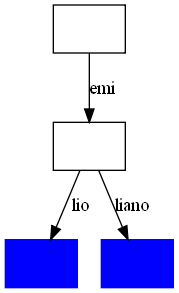
\includegraphics[scale=0.4]{./figuras/ej3/bitDeExistencia.png} }\hspace{1in} 
\centering
\subfigure[ ]{
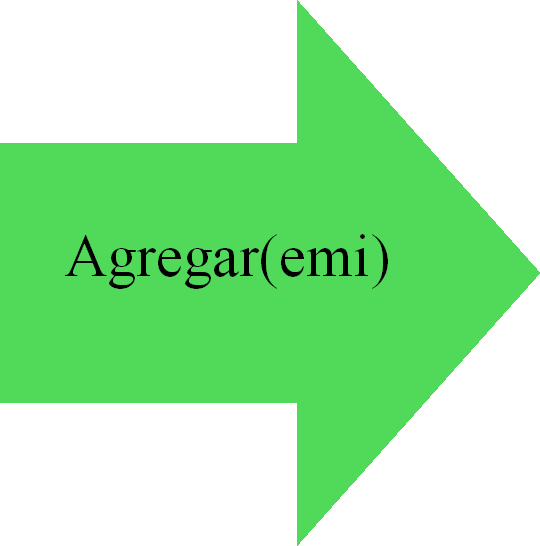
\includegraphics[scale=0.2]{./figuras/ej3/arrow3.png} }
\centering
\subfigure[La palabra emi si esta definida]{
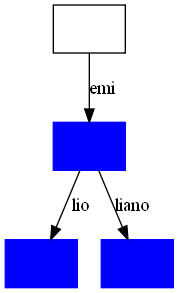
\includegraphics[scale=0.4]{./figuras/ej3/bitDeExistencia1.png} }
\setcounter{subfigure}{0}
\caption{}
\label{fig:seteaExiste}
\end{figure}

\item Para agregar un elemento hay que partir un eje y setear el bit de existe
\end{itemize}
\begin{figure}[H]
\centering
\subfigure[Bajando por el 'arbol original para agregar \"cosa\"]{
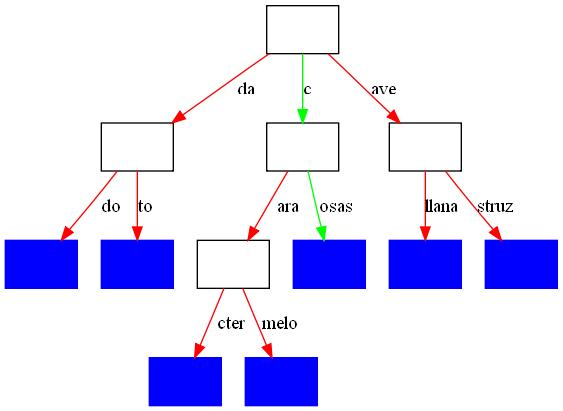
\includegraphics[scale=0.4]{./figuras/ej3/BajandoPartirYExiste.png} }\hspace{1in} 
\centering
\subfigure[ ]{
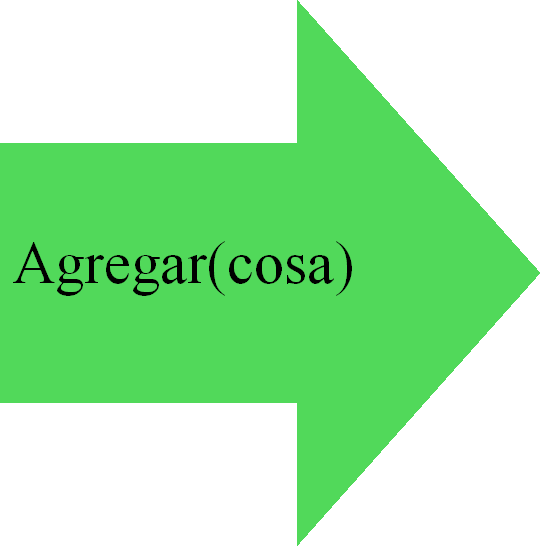
\includegraphics[scale=0.2]{./figuras/ej3/arrow4.png} }
\centering
\subfigure[Parto el eje y seteo bit de existe]{
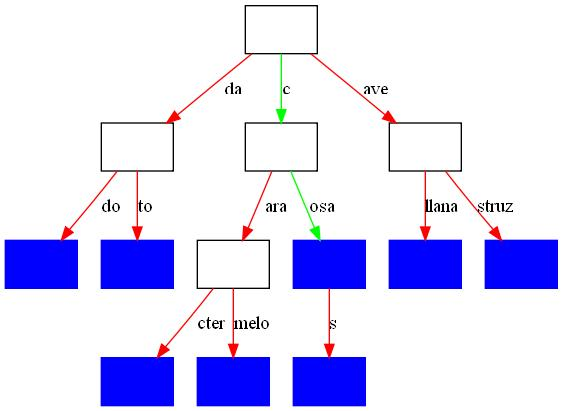
\includegraphics[scale=0.4]{./figuras/ej3/PartoUnEjeYSeteoExiste.png} }
\setcounter{subfigure}{0}
\caption{}
\label{fig:parteYSeteaExiste}
\end{figure}

Estos dos nuevos casos en realidad podemos resolverlos como derivados de los dos anteriores. Si al bajar por las ramas, la palabra formada es prefijo de la clave, y la clave es prefijo de la palabra formada, caemos en el primer caso. En este caso simplemente se setea el bit de existe al nodo en el cual caimos, como lo muestra la figura \ref{fig:seteaExiste}.
Si al bajar por las ramas, la clave es prefijo de la palabra formada y la palabra formada es m'as larga que la clave, caemos en el segundo caso. Este problema se resuelve partiendo el eje y creando un nuevo nodo en medio del eje a partir. Ahora la primer parte del eje partido apuntar'a al nuevo nodo, y la parte restante apuntar'a desde el nuevo nodo hacia el nodo en el cual caimos al bajar, como lo muestra la figura \ref{fig:parteYSeteaExiste}.
Claramente los dos primeros casos correspondientes al enunciado son excluyentes con estos dos 'ultimos casos, pues los primeros agregan solo nodos hojas, los segundos agregan solo nodos internos. Esto me asegura que el producto pedido no ser'a cambiado.

\subsection{Eliminando un elemento}
Cuando eliminamos un elemento nos enfrentamos ante los siguientes casos:
\begin{figure}[H]
\centering
\subfigure[PATRICIA]{
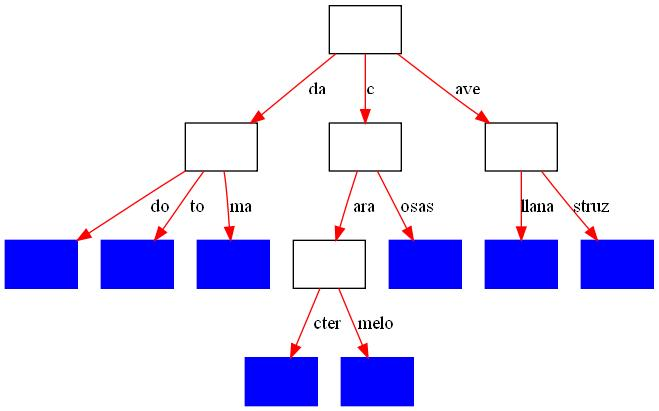
\includegraphics[scale=0.4]{./figuras/ej3/SeBorraLaHojaYNoSeMergea1.png} }
\centering
\subfigure[ ]{
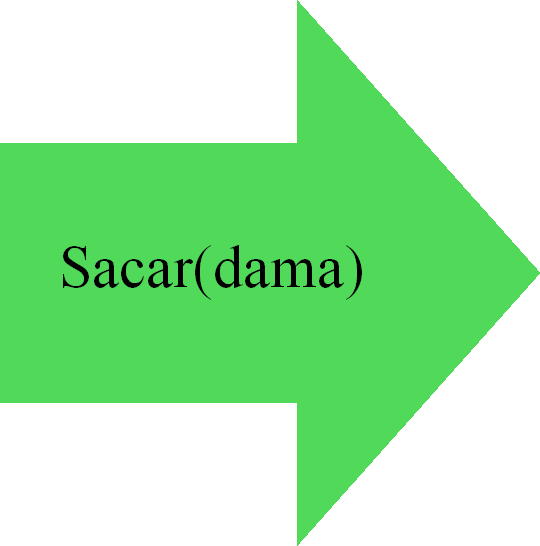
\includegraphics[scale=0.2]{./figuras/ej3/arrow5.png} }
\centering
\subfigure[Bajamos lo m'aximo posible]{
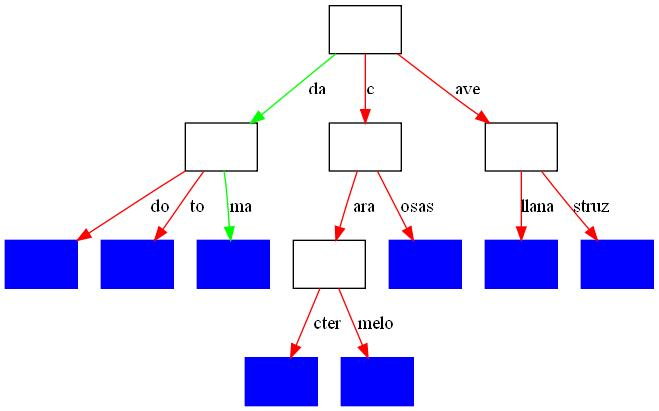
\includegraphics[scale=0.4]{./figuras/ej3/SeBorraLaHojaYNoSeMergea2.png} }
\centering
\subfigure[Patricia luego de sacar dama]{
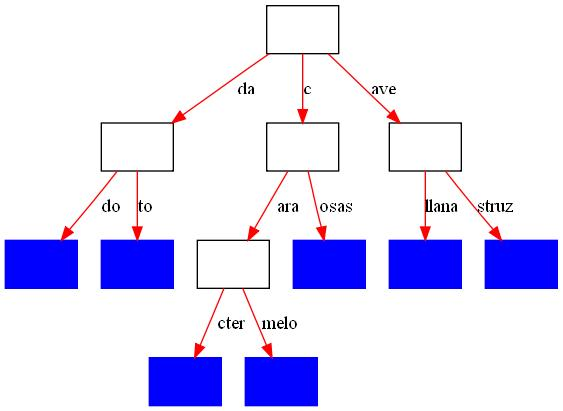
\includegraphics[scale=0.4]{./figuras/ej3/SeBorraLaHojaYNoSeMergea3.png} }
\setcounter{subfigure}{0}
\caption{}
\label{fig:borroYNoMergea}
\end{figure}

\begin{figure}[H]
\centering
\subfigure[PATRICIA original]{
\includegraphics[scale=0.4]{./figuras/ej3/patricia.png} }
\centering
\subfigure[ ]{
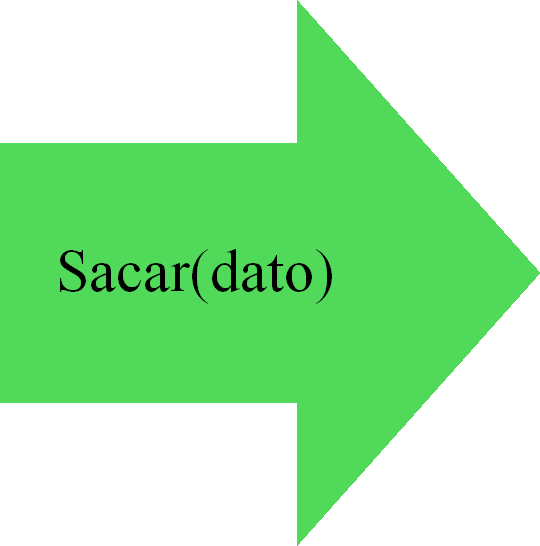
\includegraphics[scale=0.2]{./figuras/ej3/arrow6.png} }
\centering
\subfigure[Bajamos lo m'aximo posible]{
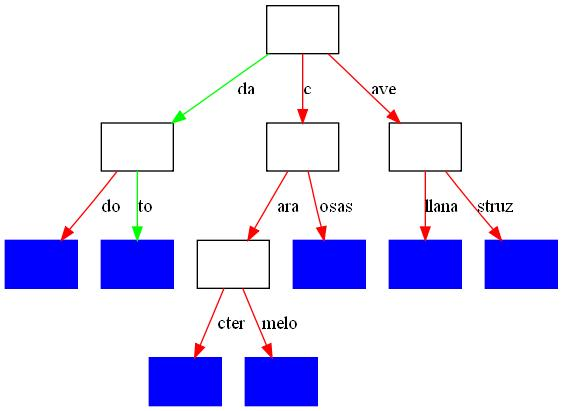
\includegraphics[scale=0.4]{./figuras/ej3/BorroHojaYMergeo1.png} }
\centering
\subfigure[Patricia luego de sacar dato]{
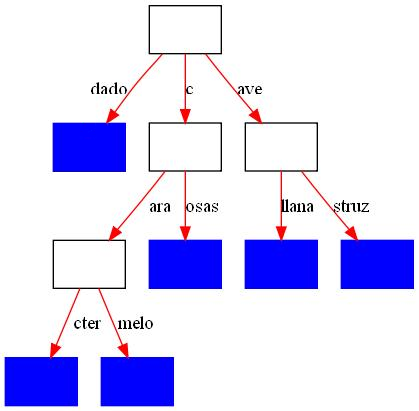
\includegraphics[scale=0.4]{./figuras/ej3/BorroHojaYMergeo2.png} }
\setcounter{subfigure}{0}
\caption{}
\label{fig:borroYMergea}
\end{figure}
Para solucionar estos casos comenzamos situ'andonos sobre la ra'iz, y bajando, al igual que agregar. Gracias a que el conjunto de entrada es libre de prefijos, sabemos que al sacar una clave siempre eliminaremos una hoja del 'arbol. De esta manera, en caso de querer eliminar una clave existente, esta siempre ser'a una hoja, como lo muestra el siguiente gr'afico:
[Grafico bajando por rama para sacar(dama)] 8
Al borrar la hoja, debemos verificar cuantos hermanos ten'ia. Si ten'ia m'as de un hermano, caeremos en el primer caso, el cual se resuelve simplemente eliminando la hoja y su eje, como lo muestra el gr'afico 6. Si, por el contrario, ten'ia solo un hermano, al borrar este nodo al padre le restar'a un solo hijo, como lo muestra la figura. Para reestablecer el invariante, como la rama hasta el nodo padre no conforma una clave definida, podemos unir el padre con su 'unico hijo. Lo hacemos simplemente borrando el nodo hijo y concatenando el eje que apunta del nodo abuelo al nodo padre con el eje que apunte del nodo padre al nodo hijo, como lo muestra el grafico 7.

Excediendo el l'imite del enunciado, nuestro algoritmo sacar podr'a tener en cuenta conjuntos de entrada que no sean libre de prefijos, sin alterar el producto pedido. Esto nos agregar'a dos casos m'as: 
\begin{itemize}
\item Para sacar un elemento hay que setear FALSE el bit de existe
\begin{figure}[H]
\centering
\subfigure[La palabra emi esta definida]{
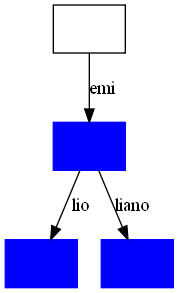
\includegraphics[scale=0.5]{./figuras/ej3/bitDeExistencia1.png} }\hspace{1in} 
\centering
\subfigure[ ]{
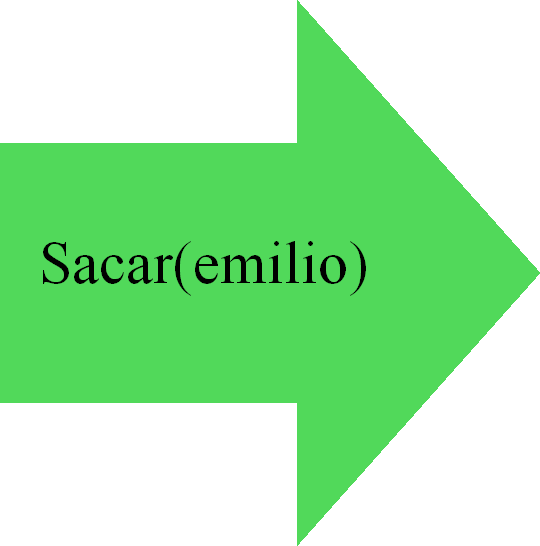
\includegraphics[scale=0.2]{./figuras/ej3/arrow7.png} }\hspace{1in} 
\centering
\subfigure[La palabra emi no esta definida]{
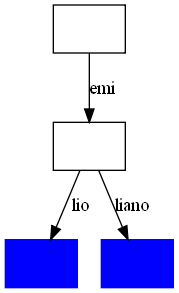
\includegraphics[scale=0.5]{./figuras/ej3/bitDeExistencia.png} }
\setcounter{subfigure}{0}
\caption{}
\label{fig:casoExtraSacarA}
\end{figure}

\item Para sacar un elemento hay que concatenar dos ejes y borrar un nodo

\begin{figure}[H]
\centering
\subfigure[La palabra emi esta definida]{
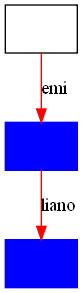
\includegraphics[scale=0.5]{./figuras/ej3/casoExtraSacar1.png} }\hspace{1in} 
\centering
\subfigure[ ]{
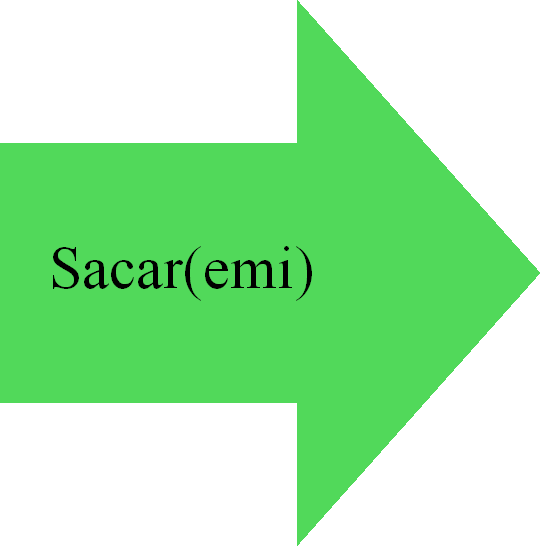
\includegraphics[scale=0.2]{./figuras/ej3/arrow8.png} }\hspace{1in} 
\centering
\subfigure[PATRICIA luego de eliminar emi]{
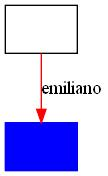
\includegraphics[scale=0.5]{./figuras/ej3/casoExtraSacar2.png} }
\setcounter{subfigure}{0}
\caption{}
\label{fig:casoExtraSacarB}
\end{figure}

\end{itemize}
Estos dos nuevos casos son consecuencia directa de los casos de entrada que no esta libre de prefijos de agregar. Luego de bajar por las ramas del 'arbol verificamos que la palabra armada es igual a la clave y el nodo existe. De esta forma nos aseguramos que la clave a borrar haya sido definida. Si el nodo a borrar es un nodo interno (no es una hoja), caemos en alguno de estos dos casos. Si el nodo a borrar tiene mas de un hijo, caemos en el primer caso. Este se soluciona seteando el bit de existencia del nodo a falso, como muestra la figura \ref{fig:casoExtraSacarA}. Si el nodo a borrar tiene solo un hijo, este es el segundo caso. Se resuelve borrando el nodo padre y concatenando el eje que apuntaba del nodo padre al nodo actual, y el eje del nodo actual al nodo siguiente, como lo muestra la figura \ref{fig:casoExtraSacarB}.
Claramente estos dos casos son excluyentes con los dos primeros correspondientes al enunciado, pues los primeros borran solo nodos internos, los segundos borran solo hojas. Esto me asegura que el producto pedido no ser'a cambiado.

\subsection{Pseudoc'odigo}
\begin{algorithm}
\caption{baja por las ramas segun una cadena s, ademas va armando la palabra que se forma durante el recorrido }
\begin{algorithmic}[1]
\PARAMS{una cadena s y otra cadena, cadenaArmada que se va a modificar}
\STATE cadenaArmada \textcolor{orange}{$\leftarrow$}  $""$
\STATE ejeAnterior \textcolor{orange}{$\leftarrow$}  \textcolor{orange}{$\bot$}
\STATE ejeActual\textcolor{orange}{$\leftarrow$}  \textcolor{orange}{$\bot$}
\STATE nodoActual \textcolor{orange}{$\leftarrow$} raiz
\STATE eje \textcolor{orange}{$\leftarrow$} eje de nodo actual que comienza con la primer letra de s
\STATE puedoBajar \textcolor{orange}{$\leftarrow$} (existe dicho eje);
\WHILE{ exista el eje \textcolor{orange}{$\wedge$} puedoBajar }
	\STATE guardamos en eje anterior el ejeActual
	\STATE guardamos en ejeActual el eje que estamos mirando ahora 
	\STATE nodoActual \textcolor{orange}{$\leftarrow$} nodo apuntado por el eje
	\STATE palabraArmada \textcolor{orange}{$\leftarrow$} palabraArmada \textcolor{orange}{++} cadena del eje
	\STATE sacar a s la parte del eje que le es prefijo
	\STATE puedoBajar \textcolor{orange}{$\leftarrow$} el eje entero era prefijo de s
	\STATE eje \textcolor{orange}{$\leftarrow$} eje del nodo actual que empieza con la primer letra de s
\ENDWHILE
\RETURN ejeAnterior
\end{algorithmic}
\end{algorithm}	

\begin{algorithm}
\caption{agrega una palabra s al conjunto}
\begin{algorithmic}[1]
\PARAMS{ la palabra s a agregar}
\STATE bajar por las ramas hasta no encontrar mas prefijo en el trie
\STATE palabraArmada \textcolor{orange}{$\leftarrow$} palabra armada durante el recorrido
\STATE acutal \textcolor{orange}{$\leftarrow$} nodo hasta donde baje
\STATE ejeActual \textcolor{orange}{$\leftarrow$} eje que apunta al nodo actual
\IF{si la palabra ya esta definida}
	\STATE no hacer nada
\ELSE
	\STATE elminar prefijos comunes de s y de palabraArmada
\IF{palabrArmada $\neq$ $""$} %\COMMENT{}
		\STATE \COMMENT{hay que partir un nodo} 
		\STATE existia \textcolor{orange}{$\leftarrow$} nodoActual.existe
		\STATE ejeActual.cadena \textcolor{orange}{$\leftarrow$} Ejactual.cadena \textcolor{orange}{-} palabraArmada  \COMMENT{dejar en el eje actual la parte que concidia con s}
		\STATE padreActual \textcolor{orange}{$\leftarrow$} nuevoNodo 
		\STATE crear eje (j) entre padreActual y nodoActual
		\STATE cadena de j \textcolor{orange}{$\leftarrow$} palabraArmada
		\STATE apuntar ejeActual a nuevoPadre 
		\IF{existia}
			\STATE poner que existe el nodoActual
		\ELSE
			\STATE poner que no existe el nodoActual
		\ENDIF
\ENDIF
\ENDIF
	\IF{ si s $\neq$ $""$}
		\STATE agregar un eje con s al nodo actual
		\STATE poner un nodo al final de ese eje, con el existe en true
	\ELSE
		\STATE setear el existe del nodo actual en true
	\ENDIF
\STATE palabras definidas \textcolor{orange}{++}
\end{algorithmic}
\end{algorithm}

\begin{algorithm}
\caption{determina si una palabras esta en el conjunto}
\begin{algorithmic}[1]
\PARAMS{ la palabra s a buscar}
			\STATE bajar por las ramas hasta que no quede mas prefijo
			\STATE palabraArmada \textcolor{orange}{$\leftarrow$} palabra armada durante el recorrido
			\RETURN palabraArmada \textcolor{orange}{==} s \textcolor{orange}{$\wedge$} el nodo existe
\end{algorithmic}
\end{algorithm}		







\subsection{Detalles de implementacion de los nodos}
Aclaraciones sobre los miembros privados de la estructura: fueron definidas 2 (dos) variables auxiliares: existe y cantElem. Si bien aislando el nodo como estructura independiente el booleano \"existe\" puede carecer de sentido, es de vital importancia a la hora de implementar el PATRICIA, ya que sin ellas no podriamos diferenciar las claves definidas de las no definidas. En cuanto a cantElem, solo existe para nodo sobre arreglos. La variable se agrega para informarnos la cantidad de hijos que tiene el nodo, y se contabiliza a medida que se agregan y sacan nodos hijos. No lo necesitamos para los nodos sobre listas, pues contamos con la funcion size de STL list.
La implementaci'on de nodos sobre arreglos cuenta con un arreglo de apuntadores a eje.
A continuaci'on explicaremos detalladamente cada funci'on referente a los nodos:
\begin{itemize}
\item constructor: inicializa el booleano existe a FALSE. En caso de nodo sobre arreglo, inicializa ademas cantElem a 0 (cero) y ademas inicializa todo el arreglo a NULL.

\item agregar: toma por par'ametro una cadena y un opcional apuntador a nodo. Adhiere un nuevo nodo al conjunto de hijos del nodo en cuesti'on. Lo hace asignandole un eje que tiene un apuntador al nuevo nodo y una cadena adjunta. Si el nodo es pasado por par'ametro, el eje apuntar'a hacia ese nodo. Caso contrario se crear'a un nuevo nodo sin nodos hijos y el eje apuntar'a hacia el nuevo nodo. Esto es as'i a causa de efectos pr'acticos a la hora de implementar el PATRICIA. Para el caso de los nodos sobre arreglos, a la i-esima letra del abecedario ingl'es le corresponde la i-esima posici'on del arreglo. En caso de los nodos sobre listas, los ejes son agregados en orden ascendiente por cadena.

\item sacar: toma por par'ametro una cadena. Borra el eje adjunto a la cadena pasada por par'ametro. No borrar'a el nodo apuntado por el eje borrado. Esto, en cambio, ser'a tarea del PATRICIA. Para el caso de los nodos sobre arreglos, borrar el eje es trivial si indexamos el arreglo  sobre la primer letra del par'ametro. En cambio, para los nodos sobre listas, se deber'a iterar sobre la lista hasta encontrar el eje a borrar.

\item pertenece: toma por par'ametro una cadena. Verifica si existe un eje adjunto a la cadena pasada por par'ametro. Para los nodos sobre arreglos, indexamos el arreglo sobre la primer letra del par'ametro y verificamos la igualdad. Para los nodos sobre listas, iteramos sobre la lista hasta encontrar la cadena buscada. Para ambos casos, si no se encuentra un eje adjunto a la cadena, se devuelve NULL.

\item getExiste: no toma par'ametros. Devuelve TRUE o FALSE, dependiendo de la existencia del nodo.

\item setExiste: toma un booleano como par'ametro. Asigna el valor del par'ametro al booleano \"existe\" dentro del objeto nodo. 

\item elemento(cadena): toma por par'ametro una cadena. Requiere que la cadena sea de longitud 1 (uno). Caso contrario devolver'a NULL. Devuelve un apuntador a eje que tiene por primer letra el parametro. Para nodo sobre arreglos, simplemente se indexa sobre la letra del par'ametro. Para nodo sobre listas, se itera sobre la lista de ejes, hasta encontrar una coincidencia entre la primer letra de la cadena adjunta al eje iterado con el par'ametro. Si no existe tal eje, se devuelve NULL.

\item elemento(entero): toma por par'ametro un entero sin signo. Devuelve un apuntador a eje. Para nodo sobre arreglos, se indexa el arreglo sobre el entero pasado par'ametro. Para nodo sobre listas, se itera sobre la lista de ejes, hasta iterar n veces, siendo n el par'ametro pasado. Si no existe tal eje, se devuelve NULL.

\item dameUno: no toma par'ametros. Devuelve un apuntador al primer eje encontrado. Para nodo sobre arreglos, se busca de 0 a 26 un eje definido. Para nodo sobre listas, se devuelve el primer elemento de la lista.

\item cardinal: no toma par'ametros. Devuelve el cardinal del nodo, entendi'endose por cardinal la cantidad de hijos que tiene. En realidad esta funci'on no hace mas que devolver el valor de la variable cantElem.

\item esHoja: no toma par'ametros. Devuelve TRUE o FALSE indicando si el nodo no tiene ningun nodo hijo o tiene alguno, respectivamente. Simplemente se compara cantElem con 0.

\item destructor: para nodo sobre arreglo, recorre el arreglo eliminando eje por eje (NO borra los nodos hijo). En caso de nodo sobre lista, no hace absolutamente nada.
\end{itemize}

\subsection{Detalles de implementacion del 'arbol PATRICIA}
Aclaraciones sobre la clase: el PATRICIA es heredero de la clase nodo y adem'as lo contiene.
\begin{itemize}
\item constructor: inicializa cantElem a 0 (cero) y la raiz, sete'andole TRUE a su valor existe.

\item destructor: hace un recorrido postorder sobre el 'arbol, borrando los nodos.

\item agregar: 
%
%    // Parametros:      cadena a agregar al PATRICIA
%	// Proposito:       le da significado a la cadena s en el PATRICIA
%    void agregar (const string& s);
%
%    // Parametros:      cadena a eliminar del PATRICIA
%	// Proposito:       le quita significado a la cadena s en el PATRICIA
%    void sacar (const string& s);
%
%    // Parametros:      cadena a verificar si pertenece al PATRICIA
%	// Proposito:       verifica si s pertenece al PATRICIA
%    bool pertenece (const string& s) const;
%
%    // Parametros:      void
%	// Proposito:       devuelve la cantidad de elementos definidos en el PATRICIA
%    unsigned int cardinal(void) const;
%
%private:
%
%    nodo* raiz;
%    unsigned int cantElem;
%    void quitarPrefijoEnComun(string& s1, const string& s2) const;
%    nodo::eje* bajar(nodo*&, nodo::eje*&, const string&, string&) const;
%    void destruirPatricia (nodo*);
%    void verPatricia (nodo*, const string&, ostream&) const;
\end{itemize}
